\section{Results}
\label{subsec:cupid-results}
A number of examples of the application of \ac{CUPID} are now provided.
Initially, a few results are presented on datasets simulated using
\textsc{Spinach}. After this, examples are provided with experimental data. In
a couple of these, comparison of the result acquired using \ac{CUPID} is
made with a spectrum acquired using \ac{PSYCHE}. For details relating to
generation of the datasets, see Sections \ref{sec:simulated-datasets} and
\ref{subsec:cupid-experimental} in the Appendix.

\subsection{``Four Multiplets''}
\label{subsec:four-mp}
\begin{figure}
    \centering
    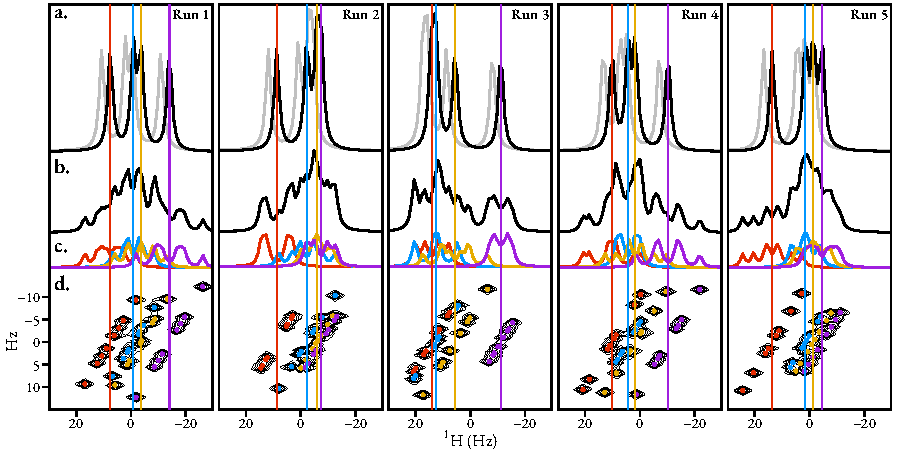
\includegraphics{four_multiplets/four_multiplets}
    \caption[
        The result of applying \acs{CUPID} to 5 instances of simulated
        \acs{2DJ} datasets with 4 heavily overlapping multiplet structures.
    ]{
        The result of applying \ac{CUPID} to 5 instances of simulated \ac{2DJ}
        datasets with 4 heavily overlapping multiplet structures.
        \textbf{a.} Black: pure shift spectrum generated by \ac{CUPID} (via the
        \ang{-45} signal).
        Grey: \ac{1D} spectrum simulated with Spinach, using the same spin
        system as was used to produce the \ac{2DJ} dataset, but with all scalar
        couplings set to \qty{0}{\hertz}. This has been offset slightly for
        clarity.
        \textbf{b.} \ac{1D} spectrum of the dataset, produced using the first
        direct-dimension \ac{FID} in the \ac{2DJ} dataset.
        \textbf{c.} Multiplet structures predicted, using a threshold $\epsilon
        = \nicefrac{\fswtwo}{\Ntwo} \approx \qty{0.98}{\hertz}$.
        \textbf{d.} Contour plot of the \ac{2DJ} spectrum in absolute-value
        mode. Coloured points denote the frequencies of oscillators in the
        estimation result.
        Coloured vertical lines denote the predicted central frequencies of
        each multiplet structure.
    }
    \label{fig:four-multiplets}
\end{figure}
A series of simulated \proton\ \ac{2DJ} datasets were generated such that
within a known region of the spectrum (\SIrange{-30}{30}{\hertz}), four ddd
multiplet structures with significant overlap exist. To achieve this, a
spin-system with 7 spins was formed, with the spins divided into 2 subsets:
\begin{itemize}
    \item Four of the spins (the ``estimated spins'') were assigned random
        resonance frequencies sampled from $\mathcal{U}(\qty{-20}{\hertz},
        \qty{20}{\hertz})$.
    \item The remaining three spins (the ``coupling spins''), were coupled to each
        of the estimated spins, with the values of the couplings randomly
        sampled from $\mathcal{U}(\qty{-10}{\hertz}, \qty{10}{\hertz})$.  The
        coupling spins were given chemical shifts such that they lay far from
        the estimated spins in the spectrum (i.e. their frequencies were $\gg
        \qty{20}{\hertz}$).
\end{itemize}
\ac{AWGN} noise was added to the \ac{FID}, with a target \ac{SNR} of \qty{30}{\deci\bel}.
A filtered sub-\ac{FID} containing only the signals from the estimated spins
was then generated using the filtering procedure described above, with
$l^{(2)}_{\unit{\hertz}} = \qty{30}{\hertz}$,
$r^{(2)}_{\unit{\hertz}} = \qty{-30}{\hertz}$.
The resulting sub-\ac{FID} was expected to comprise 32 ($4 \times
2^3$) oscillators. To assess the estimation procedure's ability, a random
integer from the range $[33, 40]$ was selected as the initial number of
oscillators. Hence, the initial guess from the \ac{MMEMPM} would comprise a
excessive number of oscillators. Due to the severe overlap of the multiplets,
application of the \ac{MDL} on the first direct-dimension signal would be
ineffective and return an under-estimate of the model order. Each \ac{FID} was
subjected to estimation, yielding the result vector $\bthstar$. Spurious
oscillators were checked for, using the criteria outlined above, with the
threshold for multiplet assignment set to the spectral resolution in the direct
dimension: $\epsilon = \nicefrac{f_{\text{sw}}^{(2)}}{\Ntwo}$. If spurious
oscillators were found, these were removed, and \ac{NLP} was run on the updated
set of parameters.

Figure \ref{fig:four-multiplets} illustrates the result achieved for 5 separate
runs of this procedure.
For each \ac{FID} generated, the method was effective at producing an
estimation result with 32 oscillators, as desired, despite the excessive number
that were present in $\bthzero$. Most of the excessive oscillators were purged
from $\bthzero$ through the \ac{NLP} procedure. When spurious oscillators did
remain\footnote{for 2 of the 5 datasets, the result after \ac{NLP} comprised 33
oscillators}, they were then detected when checking for spurious oscillators
and subsequently removed. With simulated examples, it is easy to confirm that
the pure shift spectrum generated using \ac{CUPID} agrees with the expected
pure shift spectrum; it is possible to generate the ``true'' pure shift
spectrum by simulating a pulse-acquire experiment with \textsc{Spinach}, using
a spin system with same chemical shifts, but all scalar couplings set to
\qty{0}{\hertz}.
As seen in panel a of Figure \ref{fig:four-multiplets}, the spectra produced
using \ac{CUPID} agree well with these. Panel c indicates that \ac{CUPID}
effectively resolved the multiplet structures associated with the dataset.

\subsection{Sucrose simulated}
\label{subsec:sucrose-cupid}
\note{Maybe not so impressive? Perhaps try strychnine?}
\begin{figure}
    \centering
    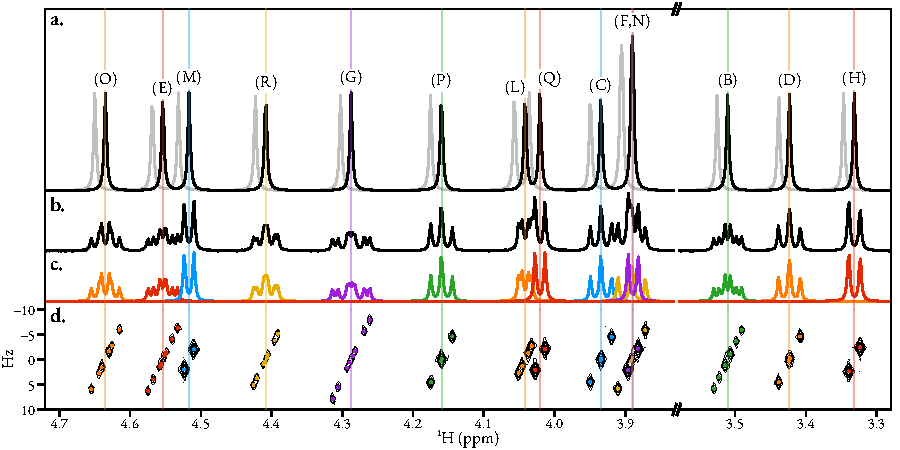
\includegraphics{sucrose_cupid/sucrose_cupid.pdf}
    \caption[
        Application of \acs{CUPID} on a simulated sucrose \acs{2DJ} dataset.
    ]
    {
        Application of \ac{CUPID} on a simulated sucrose \ac{2DJ} dataset.
        \textbf{a.} Black: the spectrum generated from \ac{FT} of the \ang{-45}
        signal. Grey: the spectrum of a simulated dataset with the same
        chemical shifts, with all scalar couplings set to \qty{0}{\hertz}.
        \textbf{b.} Conventional \ac{1D} spectrum.
        \textbf{c.} Multiplet structures assigned ($\epsilon \approx
        \qty{0.27}{\hertz}$).
        \textbf{d.} Contour plot of the absolute value mode \ac{2DJ} spectrum,
        with the locations of assigned oscillators given as coloured points.
    }
    \label{fig:sucrose-cupid}
\end{figure}
As a second example of applying \ac{CUPID} on simulated data, the chemical
shifts and isotropic scalar couplings associated with a
Gaussian\cite{Gaussian03} \ac{DFT} calculation of sucrose in a vacuum
\footnote{
It is well known that isotropic chemical shift calculations using \ac{DFT} are
typically very inaccurate. The resulting spectrum is not typical of sucrose in
the liquid state, though this doesn't really matter for assessing the
performance of \ac{CUPID}.
}
were used to construct a 2DJ dataset. \ac{AWGN} was added with a target
\ac{SNR} of \qty{20}{\deci\bel}. The CUPID procedure was applied to filtered
sub-FIDs such that the signals arising from all 22 spins were considered, though
only the regions of the dataset with the most interesting multiplet structures
are presented in Figure \ref{fig:sucrose-cupid}.

The estimation technique successfully assigned multiplet structures for all 22
multiplets in the dataset, including structures derived from two spins (F \& N)
with a \qty{0.6}{\hertz} difference in resonance frequency, approaching the
spectral resolution in the direct dimension (\qty{0.537}{\hertz}). The
pure-shift spectrum generated via the \ang{-45} signal again showed close
agreement with a 1D spectrum simulated using the same chemical shifts, with
scalar couplings set to \qty{0}{\hertz}. There are particular multiplets where
the number of oscillators fit using the estimation routine was less than the
true number. Examples of this phenomenon are exhibited in the estimates of the
multiplets for spins B \& O, which are both ddd structures. The scalar
couplings involved meant that certain oscillators were
of such similar frequencies that they were separated by significantly less than
the spectral resolution, and thus resolving these was unrealistic. For
example, there are two pairs of peaks in the spin-B multiplet which lie only
\qty{0.085}{\hertz} apart. Under-fitting in this case had a negligible impact
on the final pure shift spectrum. However there are circumstances which will be
seen in the experimental examples below where more blatant cases of under-fitting
lead to the generation of peaks in the pure shift spectrum which are noticeably
broadened.

\subsection{Quinine}
\begin{figure}
    \centering
    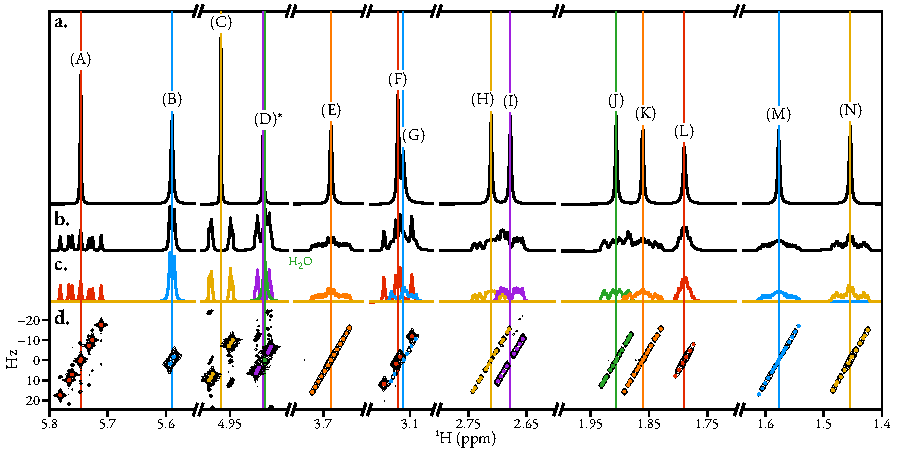
\includegraphics{quinine_cupid/quinine_cupid.pdf}
    \caption[
        Application of \acs{CUPID} on the non-aromatic regions of a quinine
        \acs{2DJ} dataset.
    ]{
        Application of \ac{CUPID} on the non-aromatic regions of a quinine
        \ac{2DJ} dataset.
        \textbf{a.} The spectrum generated from \ac{FT} of the \ang{-45}
        signal, with the signal arising from H\textsubscript{2}O (green, close
        to \qty{4.9}{\partspermillion} neglected).
        \textbf{b.} Spectrum of the first direct-dimension signal in the
        \ac{2DJ} \ac{FID}.
        \textbf{c.} Multiplet structures assigned ($\epsilon =
        \nicefrac{\fswtwo}{\Ntwo} \approx \qty{0.92}{\hertz}$).
        \textbf{d.} Contour plot of the absolute value mode \ac{2DJ} spectrum,
        with the locations of assigned oscillators given as coloured points.
    }
    \label{fig:quinine-cupid}
\end{figure}

Figure \ref{fig:quinine-cupid} illustrates the result of applying \ac{CUPID} on
a dataset generated from a sample comprising quinine (Figure
\ref{fig:structures}.a) in CD\textsubscript{3}OD,
with all signals arising from non-aromatic protons considered. The method
successfully generated a
pure shift spectrum with distinct peaks for each \textsuperscript{1}H
environment. This example also highlights an added benefit of using \ac{CUPID};
it provides the opportunity to suppress ``nuisance'' signals in the pure shift
spectrum. In this
example, an intense, broad singlet at around \qty{4.89}{\partspermillion}
was detected (see the green peak at this frequency in panel c).
The singlet was due to the presence of water in the sample and was a hindrance
due to it overlapping heavily with the multiplet structure corresponding to
spin (D). To obtain a clean singlet for spin (D) in the pure shift spectrum, the
oscillator corresponding to the water signal was simply neglected from
the parameter set used to generate the \ang{-45} signal. This concept of neglecting
nuisance signals through post-processing has been employed extensively, with
the most prominent use case being solvent suppression. The most
significant component in the data (assumed to be the solvent peak), is
determined through \ac{SVD} or some other approach, and is automatically
subtracted from the \ac{FID}\cite{Zhu1997}.
In this case, the water signal is not automatically purged from the parameter
set to construct the final pure shift spectrum, but a knowledgeable user would
be able to locate the water signal, determine that it is undesirable to include
in the pure shift spectrum, and neglect it.


As eluded to already, a few of the peaks in the pure-shift spectrum are rather
broad on account of the estimation routine under-fitting the relevant multiplet
structure. The most notable example of this phenomenon in the quinine example
comes from the peak for spin (G), where close proximity with the spin (F)
multiplet has likely compounded the task of accurately estimating the relevant
oscillators. With fewer oscillators than the true number of contributing signals
fitting a given multiplet structure, the \ac{NLP} routine will compensate by
giving the oscillators it does have at its disposal large amplitudes and
damping factors, so that they can reasonably fit multiple similar-frequency
signals. This behaviour is also exhibited by the multiplet for spin (B),
which comprises two pairs of very close signals in a dd structure. A single
oscillator is fit to each pair of signals, culminating in a broadened pure
shift peak. While linewdiths are affected by under-fitting hard-to-resolve
multiplets, the integrals of the pure shift peaks are not typically perturbed
significantly. \note{COMPUTE INTEGRALS}

\subsection{Camphor}
\begin{figure}%
    \centering%
    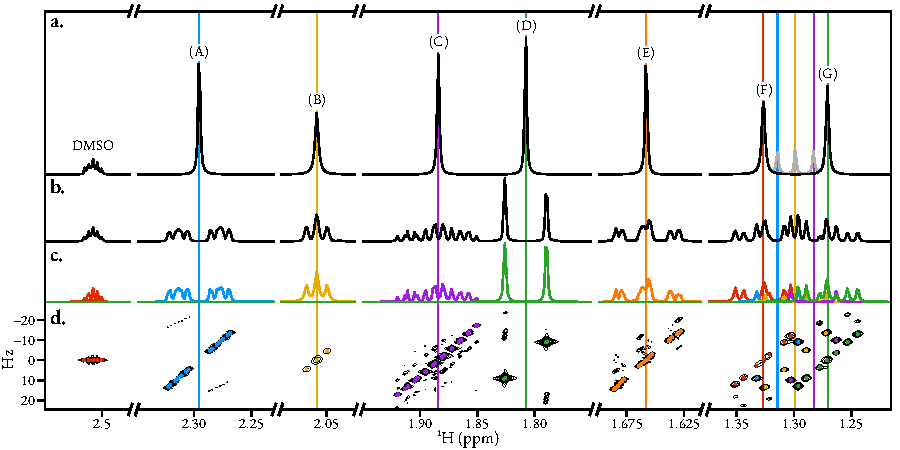
\includegraphics{camphor_cupid/camphor_cupid.pdf}%
    \caption[
        Application of \acs{CUPID} on a camphor dataset.
    ]{
        Application of \acs{CUPID} on camphor \ac{2DJ} dataset.
        \textbf{a.} Black: the spectrum generated from \ac{FT} of the \ang{-45}
        signal. Oscillators associated with strong coupling artefacts between
        spins (F) and (G) were neglected. Grey: spectrum generated without
        neglecting oscillators associated with strong coupling artefacts.
        \textbf{b.} \acs{1D} spectrum produced from the first direct-dimension
        \ac{FID} in the dataset. Note that, unlike a conventional pulse-acquire
        spectrum, strong coupling artefacts are present.
        \textbf{c.} Multiplet structures assigned ($\epsilon =
        \nicefrac{2 \fswtwo}{\Ntwo} \approx \qty{1.23}{\hertz}$).
        \textbf{d.} Contour plot of the absolute value mode \acs{2DJ} spectrum,
        with the locations of assigned oscillators given as coloured points.
    }
    \label{fig:camphor-cupid}%
\end{figure}%
\note{Are the signals that I neglect in the final pure shift spectrum definitely due to strong coupling?}
The application of \ac{CUPID} to the non-methyl regions of a \ac{2DJ}
dataset of camphor (Figure \ref{fig:structures}.c) in \acs{DMSOd6} is presented
in Figure \ref{fig:camphor-cupid}. As in the quinine case, there are instances
of underfitting poorly resolved multiplets, resulting in broadened pure shift peaks.
The peak associated with spin (B) is the most drastic case here, where 4
vicinal couplings to protons with dihedral angles of \ang{60} are present,
along with potentially more contributions from long range couplings.
This example highlights the ability of \ac{CUPID} to remove another class of nuisance peak: \emph{strong coupling artefacts}\footnote{
    As stressed in \cite{Thrippleton2005}, these are not strictly artefacts,
    but rather genuine signals, which are expected to be present in the
    \ac{2DJ} dataset. Despite this, the term is widespread in the literature.
},
which arise due to mixing effects induced by the \ang{180} pulse in the
\ac{2DJ} sequence\cite{Thrippleton2005,Wider1983}.
The effects of strong coupling lead to the presence of extra unexpected signals
which do not agree with the chemical shift of any spin associated with camphor.
An example of this is found between \SIrange{1.35}{1.25}{\partspermillion} in
the \ac{2DJ} spectrum, where artefacts associated with spins (F) and (G) are
located.
The estimation routine was able to determine parameters for
the more intense signals which comprise the strong coupling artefacts (these
are coloured blue, yellow, and purple, while oscillators associated with the
true multiplet structures for (F) and (G) are coloured red and green, respectively).
Inclusion of all oscillators extracted by the estimation routine generates the
spectrum in panel a, with the low-intensity grey peaks associated with the strong
coupling effects included. However, in much the same way as the water signal in
the quinine example could be neglected, it is trivial to construct the \ang{-45}
signal with the oscillators associated with strong coupling artefacts left out,
which produces the black spectrum.

\begin{sidewaysfigure}%
    \centering%
    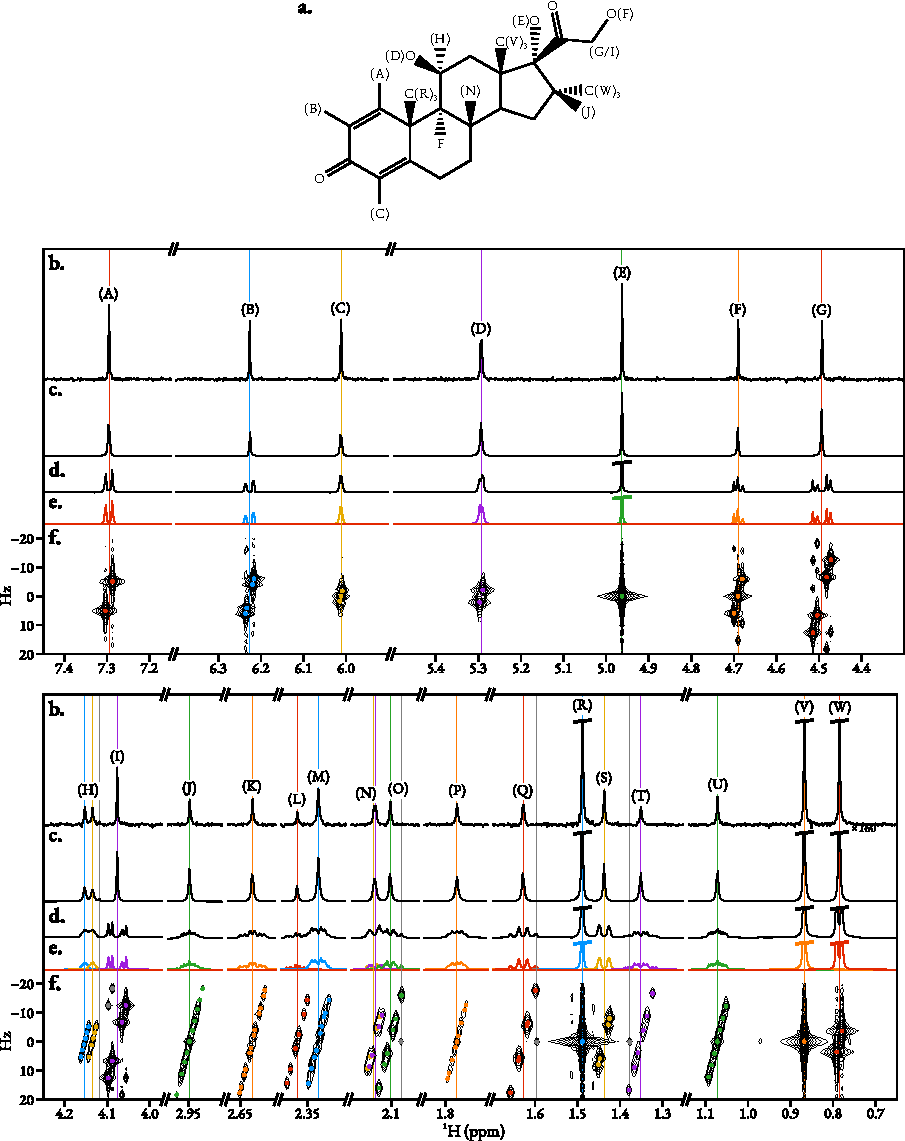
\includegraphics{dexamethasone_cupid/dexamethasone_cupid.pdf}%
    \caption[
        Application of \acs{CUPID} on a dexamethasone dataset.
    ]{
        \note{Fix magnification label.}
        Application of \acs{CUPID} on dexamethasone \ac{2DJ} dataset.
        \textbf{a.} \acs{TSE-PSYCHE} spectrum of the sample.
        \textbf{b.} The spectrum generated from \ac{FT} of the \ang{-45}
        signal.
        \textbf{c.} Conventional \acs{1D} spectrum.
        \textbf{.} Multiplet structures assigned ($\epsilon =
        \nicefrac{\fswtwo}{\Ntwo} \approx \qty{0.92}{\hertz}$).
        \textbf{d.} Contour plot of the absolute value mode \acs{2DJ} spectrum,
        with the locations of assigned oscillators given as coloured points.
    }
    \label{fig:dexamethasone-cupid}%
\end{sidewaysfigure}%
\note{Double check mp thold}

\subsection{Dexamethasone}


Figure \ref{fig:dexamethasone-cupid} shows the result of applying CUPID on a
dataset acquired from a sample dexamethasone in DMSO-d\textsubscript{6}. A
pure-shift spectrum was also acquired using the
\ac{TSE-PSYCHE} experiment\cite{Foroozandeh2018,Foroozandeh2015} for
comparison.
\ac{CUPID} generated a pure-shift spectrum with overall excellent agreement
with the \ac{TSE-PSYCHE} spectrum. Certain multiplet structures in the spectrum exhibit
splitting in the direct dimension, on account of heteronuclear couplings to
\textsuperscript{19}F. Most notable are those derived from spins (D), (H) \& (O). For the (D) multiplet, the
magnitude of the heterocoupling is very small such that assigning these to
separate oscillators was not achievable.
For the spin (N) multiplet, two separate structures were successfully assigned
(see the orange and green multiplets around \qty{2.1}{\partspermillion}).
The estimation routine was unsuccessful at accurately estimating the structure
associated with spin (H), where a severe under-fitting occurred. An under-fitting
of this structure even occurred when the estimation was re-run using
considerable over-estimation of the model order, with most oscillators in the
initial guess being purged during the \ac{NLP} procedure.
The spin (H) multiplet provides an extreme example line-broadening in the pure
shift spectrum on account of under-fitting. The most downfield peaks in the
CUPID spectrum (corresponding to aromatic and hydroxyl protons) also appear to
be noticeably broadened relative to their PSYCHE equivalents. This is also
probably due to under-fitting of the relevant multiplet structures, though to a
far less noticeable extent than for spin H. \note{Any other reason why this
might be so?}

\subsection{Estradiol}
\begin{figure}
    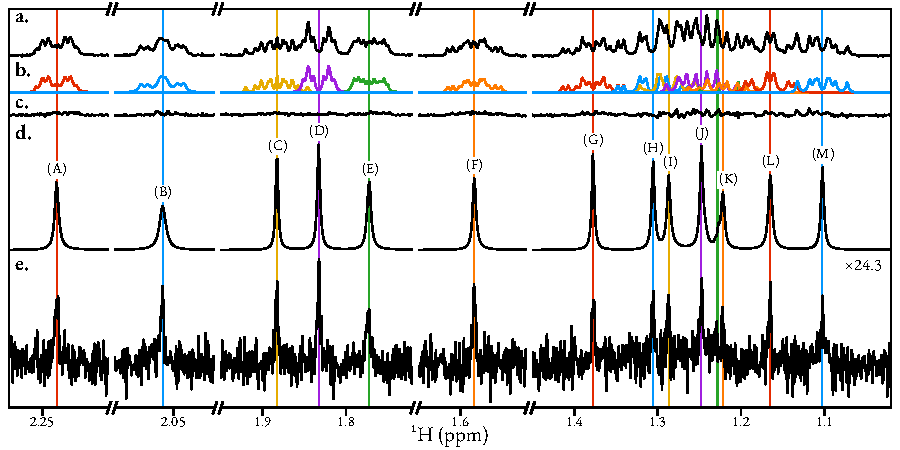
\includegraphics{estradiol_cupid/estradiol_cupid.pdf}%
    \caption[
        Application of \acs{CUPID} on a 17\textbeta-estradiol dataset.
    ]{
        Application of \acs{CUPID} on \ac{2DJ} dataset of 17\textbeta-estradiol
        in \acs{DMSOd6}.
        \textbf{a.} Spectrum of the first direct-dimension \ac{FID} in the
        \ac{2DJ} dataset.
        \textbf{b.} Multiplet structures assigned ($\epsilon =
        \nicefrac{\fswtwo}{\Ntwo} \approx \qty{2}{\hertz}$).
        \textbf{c.} The residual between the spectrum in panel a and the lines
        in panel b.
        \textbf{d.} The pure shift spectrum generated using \ac{CUPID}.
        \textbf{e.} \acs{PSYCHE} spectrum of the sample see Figure
        \ref{fig:psyche} for details on the pulse sequence. The spectrum has
        been scaled such that the maximum is of the same magnitude as the
        corresponding point in the \ac{CUPID} spectrum.
    }
    \label{fig:estradiol-cupid}%
\end{figure}

A final showcase of \ac{CUPID} is provided by Figure \ref{fig:estradiol-cupid}, where a low concentration (\qty{2}{\milli\molar}) sample of 17\textbeta-estradiol (Figure \ref{fig:structures}.
